

\chapter{Introduction}

%\label{chap:GettingStarted}
\section{Overview}
The introduction of a Co-operative Society Management System marks a significant leap
in the efficient and organized management of Co-operative societies. Co-operative
societies play a vital role in various sectors, including agriculture, finance, and housing,
by fostering collaboration among members and promoting economic development.
However, managing the diverse functions and operations of these societies can be
complex and demanding. This introduction provides an overview of the purpose, features,
and benefits of such a system.

\subsection{Purpose}
The Co-operative Society Management System is designed to address the unique needs
and challenges faced by Co-operative societies. Its primary purpose is to streamline and automate the administrative, financial, and member-related processes within a Cooperative society, ultimately enhancing its efficiency, transparency, and overall
performance.

% \section{Motivation}

% \subsection{Image Processing}






\section{Background}
The concept of Co-operative societies has a deep-rooted history in Bangladesh, dating back to the pre-independence period and gaining significant momentum in the post-independence era. Here's a brief background on Co-operative societies in Bangladesh: 

Pre-independence Period: Co-operative societies in what is now Bangladesh can trace their origins to the British colonial period. During this time, Co-operative movements began to take shape, primarily in rural areas. These early Co-operatives aimed to address the economic challenges faced by farmers and rural communities. However, the concept remained somewhat limited in scope. Post-independence Era: After gaining independence from Pakistan in 1971, Bangladesh faced numerous socio-economic challenges. Co-operatives were seen as a means to empower rural communities, alleviate poverty, and promote economic development. The government of Bangladesh began to actively promote and support Co-operative initiatives as part of its socioeconomic development strategy. 

Co-operative societies in Bangladesh have a diverse history and have played a significant role in addressing rural and urban development challenges. With ongoing efforts to overcome challenges and promote transparency, Co-operatives continue to be a valuable instrument for socio-economic development and poverty reduction in the country.


\section{AIM}
The aims of Co-operative societies in Bangladesh are multifaceted and are aligned with socioeconomic development, poverty reduction, and the empowerment of various segments of society.
Here are the primary aims of Co-operative societies in Bangladesh:

a. Poverty Alleviation

b. Rural Development

c. Agricultural Advancement

b. Financial Inclusion

c. Empowerment of Women

d. Housing and Urban Development

e. Entrepreneurship Development

f. Social Welfare

g. Community Building

h. Good Governance

Co-operative societies in Bangladesh have a broad spectrum of aims, all of which are geared
towards socio-economic development, poverty reduction, and the empowerment of individuals
and communities. They play a crucial role in addressing the diverse needs of their members and
contribute to the overall development of the country

\section{Motivation}
The motivation behind developing a Co-operative Society Management System stems from the recognition of several pressing needs and challenges within Co-operative
societies. Here are the primary motivations:

1. Efficiency Enhancement: Traditional methods of managing Co-operative societies
often involve manual paperwork, which can be time-consuming and error-prone. The
motivation is to streamline operations and reduce administrative burdens by automating
various tasks, ultimately improving efficiency.

2. Transparency and Trust: Co-operative societies rely on the trust and cooperation of
their members. By implementing a management system, societies aim to enhance
transparency in financial transactions, member interactions, and decision-making
processes. This increased transparency fosters trust among members and stakeholders.

3. Compliance and Reporting: Many Co-operative societies are subject to regulatory
requirements and reporting standards. A management system simplifies compliance by generating accurate financial reports and statements, making it easier to adhere to legal obligations.

4. Member Empowerment: Co-operative societies exist for the benefit of their
members. By providing an online platform for members to access their account
statements, apply for loans, and engage in discussions, the system empowers members
and improves their overall experience.

5. Data Security: Data security and privacy are paramount. With the rise in cyber threats, a motivation for implementing a management system is to ensure that sensitive member and financial data is securely stored, reducing the risk of data breaches.

6. Scalability: As Co-operative societies grow, the need for efficient management
becomes more critical. The system allows for scalability, enabling societies to
accommodate a larger membership base and increasing volumes of financial transactions.

7. Cost Reduction: While there may be an initial investment in implementing the system,
the long-term motivation is cost reduction. By automating tasks and reducing the need for extensive manual labor, Co-operative societies can save both time and money.
The motivation for a Co-operative Society Management System lies in its ability to
address the unique challenges faced by Co-operative societies, improve operational
efficiency, enhance transparency, ensure accurate financial management, empower
members, and ultimately contribute to the long-term sustainability and success of these
Co-operative organizations. 

\begin{figure}
    \centering
    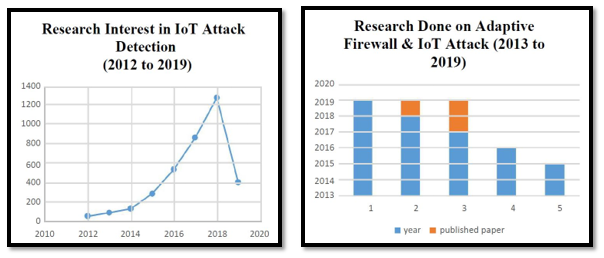
\includegraphics[scale=0.5]{Chap1/motivation.PNG}
    \caption{Research Interest in Field of IoT}
    \label{fig:motivation}
\end{figure}

 In figure \ref{fig:motivation} shows the existing research interest in IoT Attack Detection which is increasing day by day for last few years whereas for detecting attack concept of Adaptive Firewall is not so common and used term in this field. This drives us motivated to design adaptive firewall for attack detection and to block illegitimate traffic on IoT Network Model.
\section{Objective}
%The Overview goes here \cite{r1}.
IoT network model and devices are vulnerable to different kind of attacks. These attacks may vary to different category, so have different approach to detect and block them. The goal of this research is to study and identify potential IoT security attacks, detect and mitigate them by using Adaptive firewall concept. Additionally, machine learning should be considered for classifying attacks and identifying attacks \cite{c4}.
Specific goals of this thesis that should be mentioned:

\begin{itemize}
    \item Analyze network traffic to detect the malicious ones that tries to hamper the network.
    \item Find the characteristics of perception layer’s attack to identify specific attacks.
    \item Extract features from the generated traffic datasets to train machine learning classifiers and apply them to recognize attacks.Propose a centralized attack detection model.
    \item Design a rule based and ANN based FIS to help SDN controller to evaluate specific attack probability and block the suspicious ones.
    \item Maintaining the performance of the network.
\end{itemize}

This proposed model also answers the following questions:
\begin{enumerate}
    \item What are the major challenges that have guided security in IoT?
    \item What is the best attack detection way for IoT network model?
    \item Is there any generalized approach for detecting different layer attack?
    \item What is the best way to detect a single layer attack?
\end{enumerate}

\section{Assumptions \& Limitations}
Though a centralized and efficient model has been proposed to detect attacks on IoT network, it has limitations on which further studies should be done:
\begin{itemize}
    \item No approach has been mentioned for network and application layer security.
    \item No real time data has been used for the traffic analysis.
    \item Here feature Extraction and Selection method has been analyzed but no implementation has been shown.
    \item No comparison among different IDS model has been analyzed so can’t be declared it as the optimal way. 
    \item No performance measure of used Classifier is evaluated here.
\end{itemize}

\section{Research Outline}
Rest of the report is structured as follows: In \textbf{Chapter \ref{chap:2}} a literature study on related work is given including explanations for the most important terms used in this thesis-basic concept and architecture of IoT Network Model, Attacks on IoT, Concept and architecture of SDN, different model of IDS, Concept of Firewall has been discussed through this chapter. \textbf{Chapter III}  introduces system model including system architecture, algorithm and flowchart of working procedure of entire system model. \textbf{Chapter IV} explains the details of traffic analysis techniques, Feature Extraction and Selection mechanism and tools for this mechanism and reasoning how these mechanisms work for our model. \textbf{Chapter V} discusses about the simulation and model performance, to analysis result of the model it describes the basic mechanism of attack detection like Fuzzification, NSL KDD dataset, FIS, Defuzzification,Simulation and confusion matrix. Lastly in \textbf{Chapter VI} future work and conclusion is mentioned. 

\section{Limitation}
Bla bla bla
\label{sec:EffSearch} 
\index{Search engines!using effectively} %index will be created
%The rest of this report is organized as follows.

